\chapter{Forward Kinematics}

To model the movements of the end effector of a kinematic chain, a forward kinematic analysis is needed. This means, that the position of the endpoint in the operational space needs to be described by the kinematic equations with the joint space as input. The non-linear kinematic equations map the joint parameters to the configuration of the robot system.   This results in a pure geometrical description of motion  by means of position, orientation, and their time derivatives.

\section{Approach}
A serial-link manipulator consists of links in a chain connected by joints. 
A link is a rigid body, defining the spatial relationship between two following axes.
For describing the serial-link mechanism geometry the Denavit Hartenberg notation is one possible approach.
It gives a description of a manipulator for kinematic solutions, Jacobians, dynamics, motion planning and simulation. 
This description can be obtained through a five step algorithm:\cite{ConstantinForwardKA}

\section{Numbering the joints and links}
A serial link robot with n joints has $n+1$ links. 

\paragraph{numbering of links}
The numbering scheme for links starts at $(0)$ with the fixed grounded base and then increases sequentially up to $(n)$ for the end effector.

\paragraph{numbering of joints}
The numbering scheme for joints starts at $(1)$ with the joint connecting the first movable link to the base and then increases sequentially up to n.

\paragraph{relation between links and joints}
Link $(i)$ is connected to its 
\begin{itemize}
	\item lower link $(i-1)$ at its proximal \cite{proxdist} end by joint $(i)$
	\item upper link $(i+1)$ at its distal \cite{proxdist} end by joint $(i+1)$
\end{itemize}

\paragraph{Joint and link numbering in Fanuc 210F}

This numbering scheme can be applied to the Fanuc 210F (see \ref{fig:LinksANDJoints210F}) 


\begin{figure}[H]
	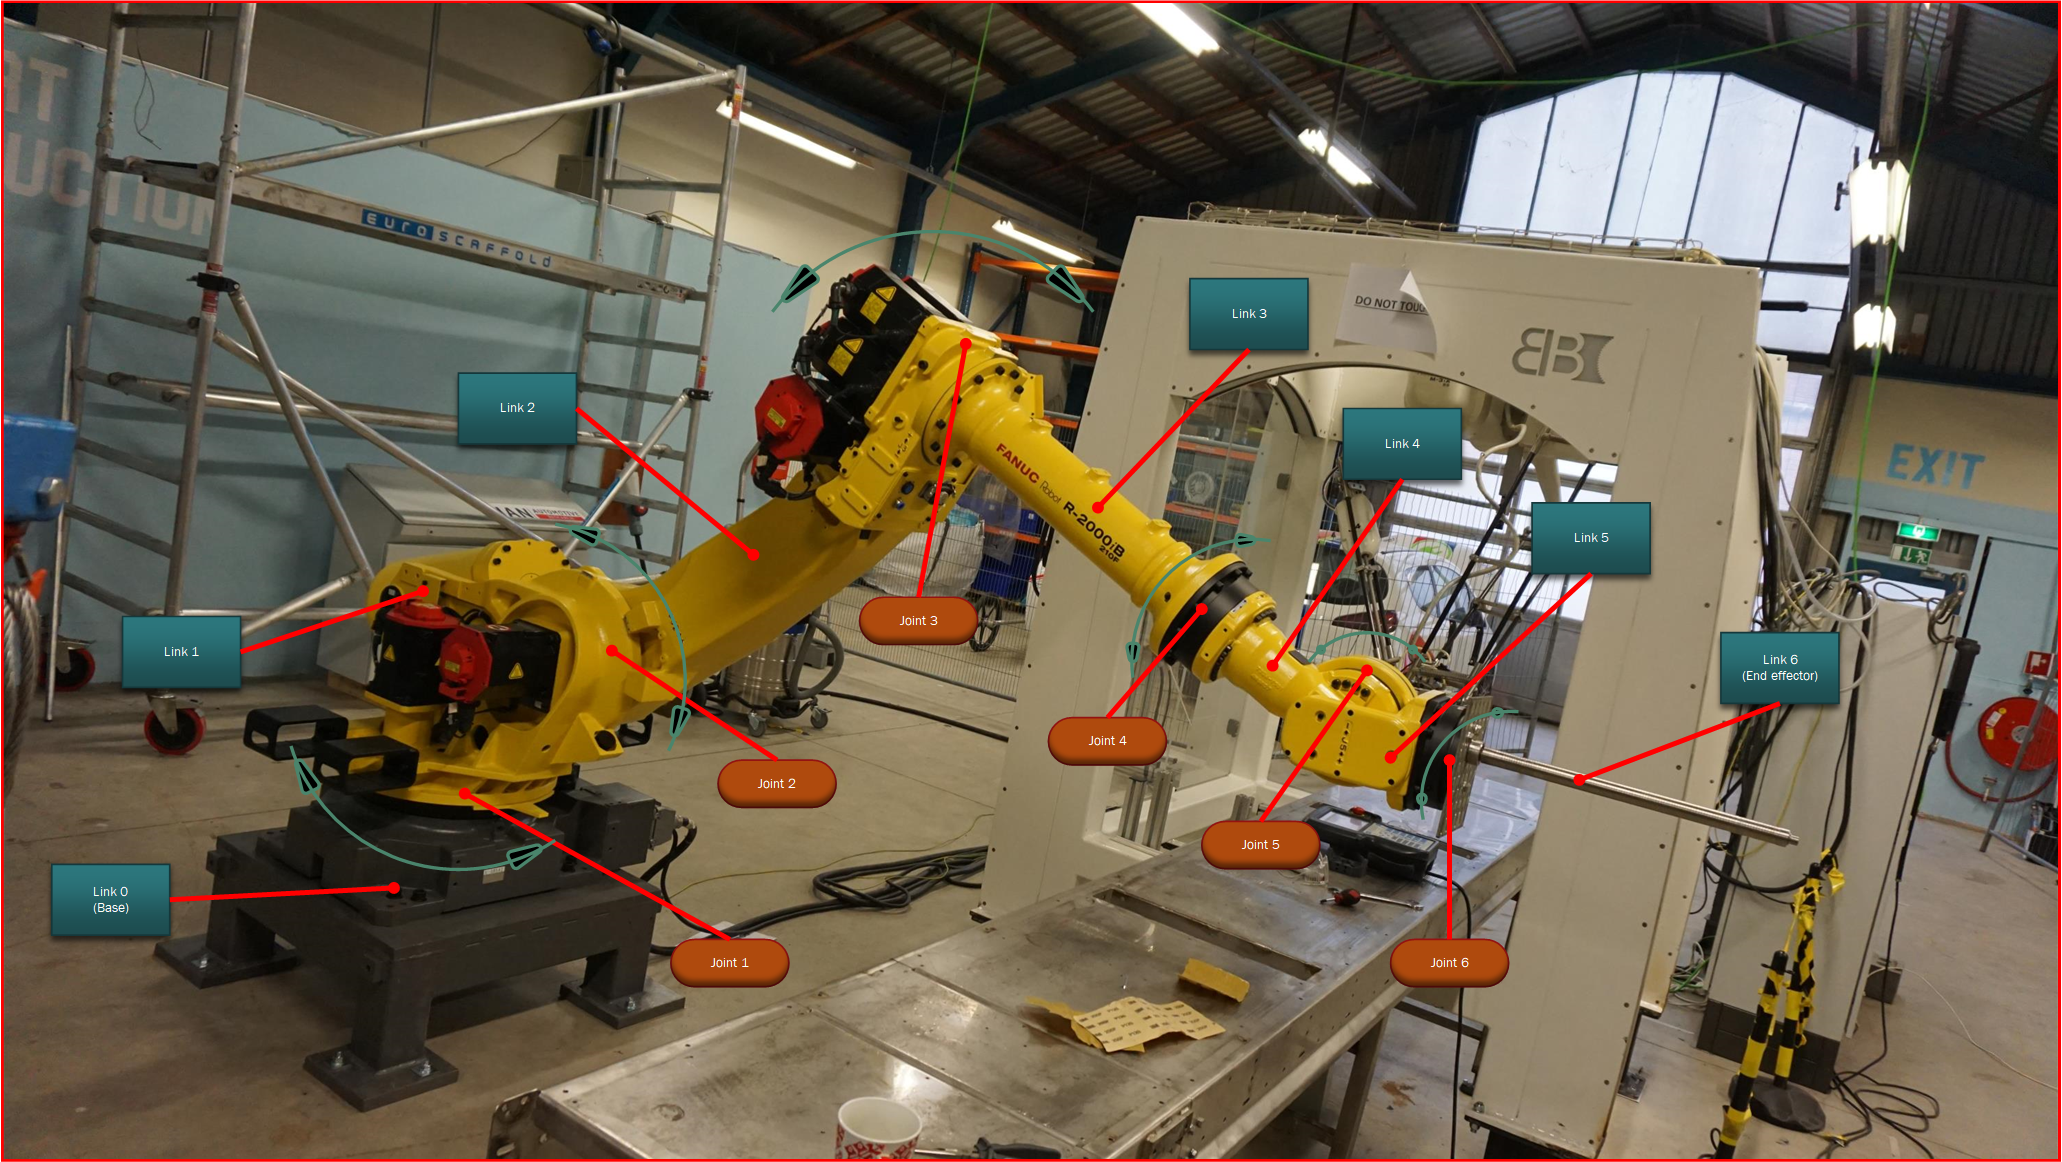
\includegraphics[
	width=1\linewidth,
	center,
	keepaspectratio,
	]{linksANDjoints/linksAndJoints}
	\caption{Links (turquoise) and joints (orange) in the FANUC 210F}
	\label{fig:LinksANDJoints210F}
\end{figure}



\section{local coordinate reference frames}
With the Denavit-Hartenberg convention, local coordinate frames can be attached to the far end of the links $ (i) $ and their accompanying joints $ (i+1) $.
Each link $(i)$ is described relative to the pose of the preceding link.

%\paragraph{Assignation of coordinate frames}


\paragraph{Assignation of $z_i$ axes}

With the DH-notation, the $z_i$ axes are assigned to link $(i)$.
Two cases need to be considered: %regarding joint $(i+1)$:
\begin{itemize}[wide=\parindent]
	\item[\textbf{revolute:}] $z_i$ is the axis of revolution of joint $(i+1)$
	\item[\textbf{prismatic:}] $z_i$ is the axis of translation of joint $(i+1)$
\end{itemize}
%of joint $(i+1)$
This means, that joint $z_i$ turns around axis $z_i$.

\paragraph{Direction of rotation}
With the direction of the $z_i$-axis, the direction of positive rotation around joint $(i+1)$ is also given by the right hand rule (see \cite{Angela_U1S2P1} at 10:35). This means, the direction of positive rotation is counter-clockwise around the $z_i$-axis.
With predictive choice of the direction of positive rotation, the direction of the z-axis can be chosen in order to minimize the DH-parameters (insert source here)

\paragraph{$z_i$ axes in Fanuc 210F}
As described above, the $z_i$ axes can be attached to the Fanuc 210F (see figure \ref{fig:zi_Axes}).


\begin{figure}[H]
	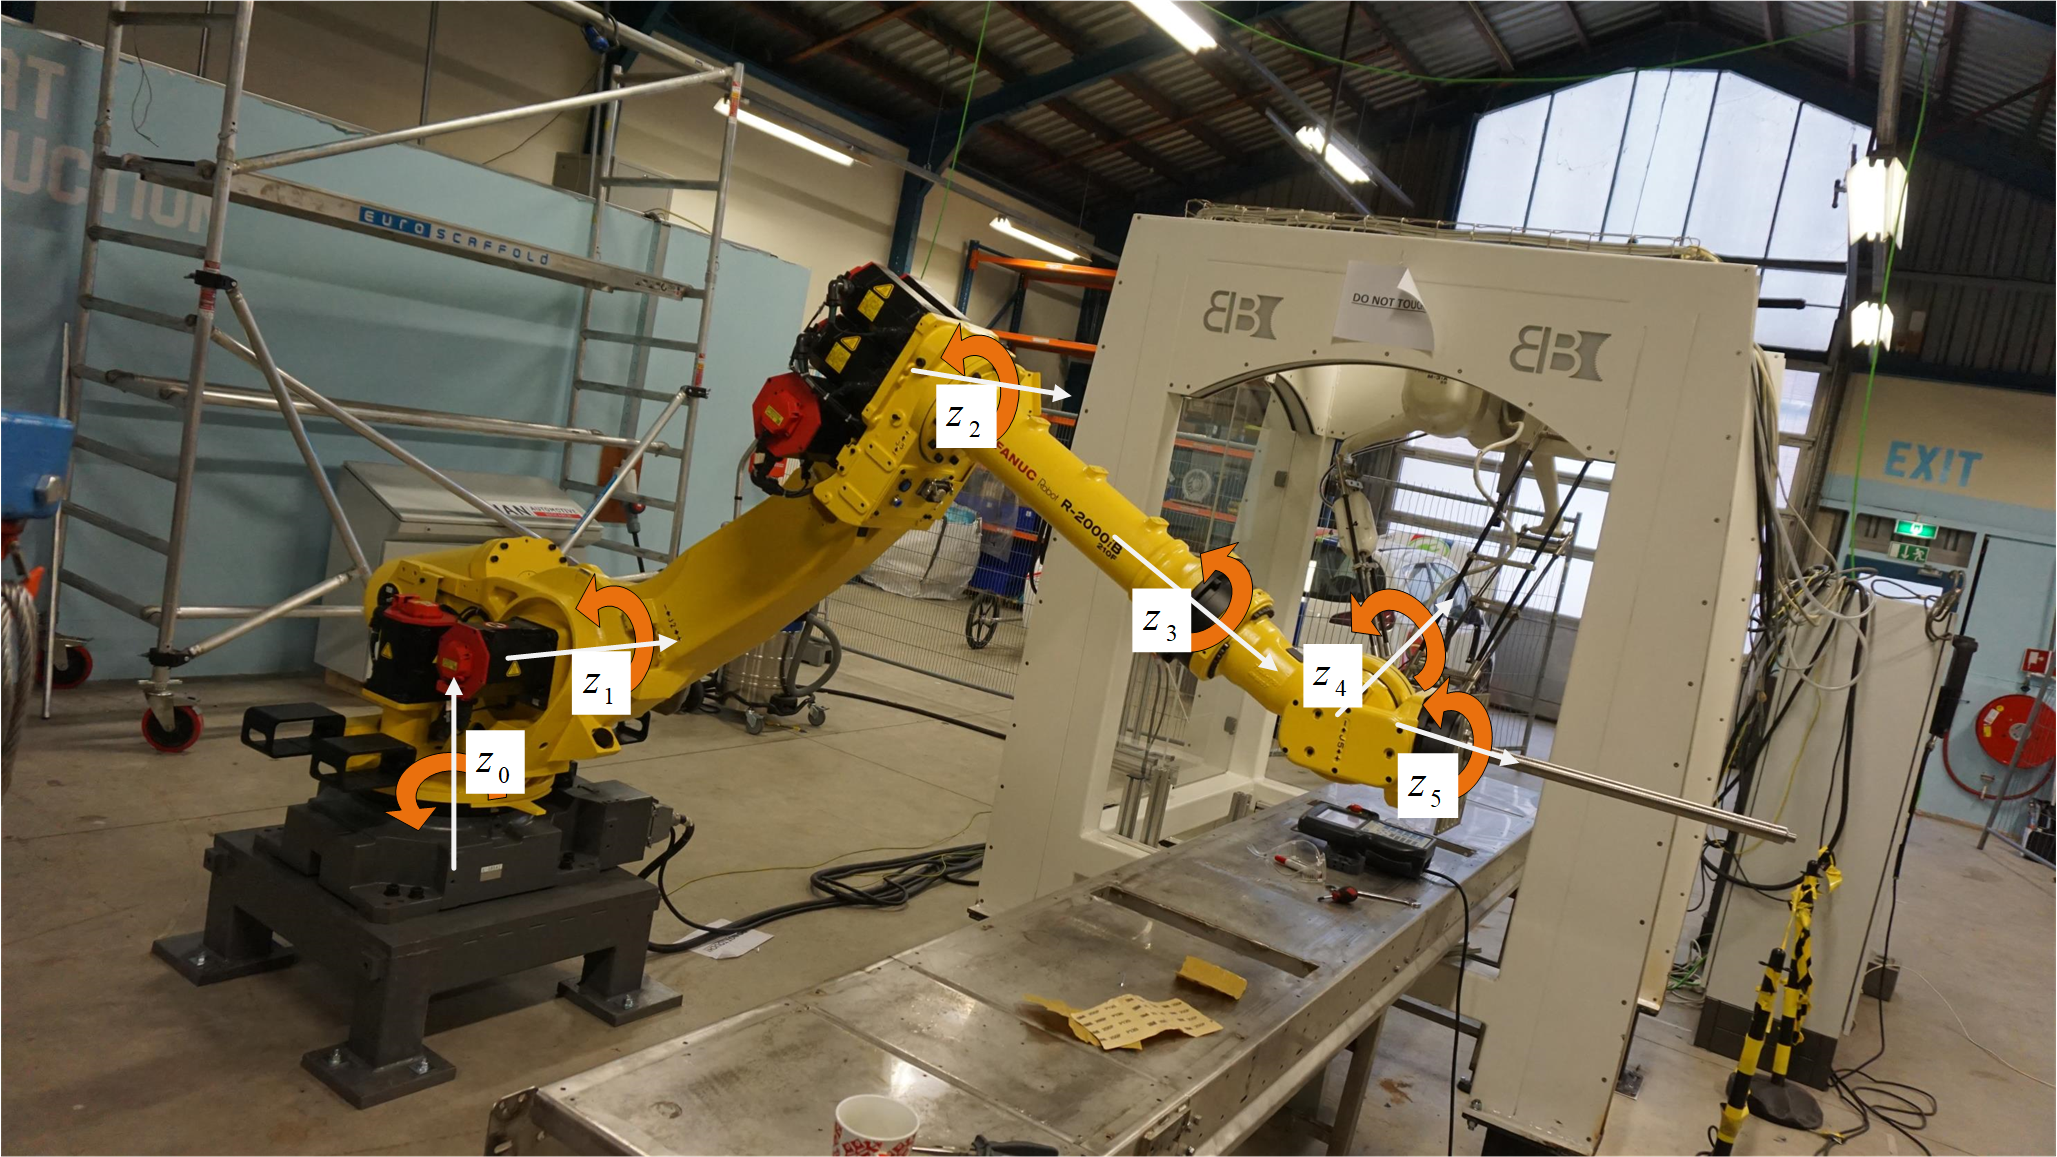
\includegraphics[
	width=1\linewidth,
	center,
	keepaspectratio,
	]{coordinateFrames/z_axes}
	\caption{$z_i$ axes on the Fanuc 210F with the direction of positive rotation (orange)}
	\label{fig:zi_Axes}
\end{figure}

The positive direction of the triples $z_1$, $z_2$, $z_4$ and $z_0$, $z_3$, $z_5$, was chosen to make sure, the x-axis would always have the same direction for parallel joints. 

\paragraph{Base frame}

The base frame $(0)$ can be chosen nearly arbitrarily. The origin of the base frame can be any point on $z_0$. For simplicity, the origin of frame$(0)$ can be put into joint$(1)$.  Usually, the x-axis of the base frame is chosen, so that it points in the direction of the \ac{EOAT} in default position according to its base, \cite{DenavitHartenbergKonventionen} but can be chosen in any convenient manner \cite{SpongDynContr}.

\paragraph{Assignation of frames $(i)$}

Starting from frame $(0)$ in an iterative process, frame $(i)$ can be set up using frame $(i-1)$.

Three cases regarding the relationship of axes $z_{i-1}$ and $z_i$  need to be considered when setting up frames:
\begin{itemize}[wide=\parindent] %option solves alignment problem for item label %https://tex.stackexchange.com/questions/246394/alignment-of-labels-in-itemize-with-text-of-document 
	\item[\textbf{Non coplanar:}] Axes don't intersect and are not parallel. Line containing the common normal $z_{i-1}$ to $z_i$ defines $x_i$-axis and the point of intersection with $z_i$ is the origin of frame $(i)$
	\begin{enumerate}[label=\emph{\alph*)}]
		\item find common normal of the joint axes
		\item put origin in intersection of normal with joint axis
		\item put $z_i$ axis in the joint axis
		\item $x_i$ points in direction of the common normal, facing away from frame $(0)$
		\item add $y_i$ according to right hand rule
	\end{enumerate}
	\item[\textbf{Parallel:}] Axes are parallel. Line containing the normal through origin of frame $(i+1)$ and the $z_i$-axis defines the $x_i$-axis which is directed from origin of frame $(i)$ toward the distal joint. The point of intersection of common normal with $z_i$-axis gives the origin of frame $(i)$. % found a mistake here with common normal in \cite{ConstantinForwardKA} witht he help of \cite{SpongDynContr}. The x-axis should point towards next joint, but he says, should point towards last joint, but does it actually the other way around.
		\begin{enumerate}[label=\emph{\alph*)}]
		\item look for normal originating from distal joint
		\item put origin in the intersection of the normal with the joint axis
		\item put the $z_i$ axis in the joint axis of the link $(i+1)$ 
		\item $x_i$ points follows the common normal with the distal joint, pointing towards the distal joint
		\item add $y_i$ according to right hand rule
	\end{enumerate}
	\item[\textbf{Intersecting:}] Axes are intersecting. Line containing the normal to the plane formed by axes $z_{i-1}$ and  $z_i$ gives the $x_i$-axis with positive direction chosen arbitrarily. Point of intersection of  axes $z_{i-1}$  and  $z_i$ is the origin of frame $(i)$.
		\begin{enumerate}[label=\emph{\alph*)}]
		\item put origin in intersection point of the axes
		\item put the $z_i$ axis in the joint axis of the link $(i+1)$
		\item $x_i$ is perpendicular to both joint axes
		\item add $y_i$ according to right hand rule
	\end{enumerate}
\end{itemize}

\paragraph{Assignation of \ac{EOAT} frame}
As there is no distal joint for the \ac{EOAT} frame, the steps for this frame are different:

\begin{enumerate}[label=\emph{\alph*)}]
	\item put origin on axis of proximal joint 
	\item axis $z_i$ follows direction of $z_{i-1}$
	\item $x_i$ can be chosen arbitrarily, but is usually determined by screw holes
	\item add $y_i$ according to right hand rule
\end{enumerate}

\paragraph{local coordinate reference frames on the Fanuc 210F}

As described above, the local coordinate reference frames can also be attached to the Fanuc 210F as seen in \ref{fig:RefFrame}. 

\begin{figure}[h]
	\includegraphics[
	width=1\linewidth,
	center,
	keepaspectratio,
	]{coordinateFrames/CoordinateFrames}
	\caption{Coordinate reference frames for Fanuc 210F}
	\label{fig:RefFrame}
\end{figure}

\paragraph{frame 0 (Base)}
The frame mapping starts with the base frame. For the base frame the z-axis is given through joint $j_1$. Origin of frame 0 is put into joint 1.
The x-axis is chosen to point in direction of of the \ac{EOAT} in standard pose. For standard pose see \ref{fig:StandardPose}.
This pose will also be chosen for alignment of all distal frames.

\begin{figure}[h]
	\includegraphics[
	width=1\linewidth,
	center,
	keepaspectratio,
	]{coordinateFrames/standardPose}
	\caption{Standard pose of the robot}
	\label{fig:StandardPose}
\end{figure}

\paragraph{frame 1}
For frame 1, the z-axes are not coplanar. 
Because of that, the  $z_0$-axis is extended until a common normal can be found that intersects with $z_i$ to define the origin $O_1$.
$x_1$ departs from $O_1$ along the common normal.
$y_1$ is added according to the right hand rule.

\paragraph{frame 2}
As seen, in image \ref{fig:zi_Axes}, axes $z_2$ and $z_1$ are parallel. $O_2$ can be found at the intersection of the normal through $O_1$ with $z_2$. $x_2$ follows the common normal with joint 4.
$y_2$ is added according to the right hand rule.

\paragraph{frame 3}
Joint 3 and joint 4 are not exactly aligned (see image \ref{fig:StandardPose}), which prevents the z-axes to intersect. That's why axes $z_3$ and $z_2$ are not coplanar. 
$z_3$ runs parallel through the link 3, due to the orientation of the rotational axis.
As the common normal between $z_3$ and $z_2$ defines $x_3$, which in turn gives $O_3$, the origin can be found far away from the physical position of the joint.
$y_3$ is added according to the right hand rule.

\paragraph{frame 4}
Joint 5 lies in line with joint 4.
As $z_3$ follows this line, the axes  $z_4$ and $z_3$ intersect in the center of joint 5, which gives $O_4$. 
$x_4$ leaves the plane spanned by  $z_4$ and $z_3$ perpendicular.
The positive direction of $x_4$ is chosen to be similar as in frame 3 for simplicity.
$y_4$ is added according to the right hand rule and points in direction of frame 3.

\paragraph{frame 5}
As $z_5$ lies  in line with $O_4$, the axes  $z_5$ and $z_4$ intersect in $O_4$ which puts $O_5$ at the same position as $O_4$.
$x_5$ leaves the plane spanned by  $z_5$ and $z_4$ perpendicular.
The positive direction of $x_5$ is chosen to be similar as in frame 4 for simplicity, which puts $x_5$ and $x_4$ on top of each other. 
$y_5$ is added according to the right hand rule and as $z_5$ is turned 90 degrees relative to $z_4$ around $x_{4,5}$, $y_5$ is turned 90 degrees relative to $z_4$ around $x_{4,5}$ as well.

\paragraph{frame 6 (EOAT)}
$z_6$ lies in line with $z_5$ and is consequently parallel.
as there are no distal joints, to reference $x_6$, it can be chosen arbitrarily. 
For simplicity, it is chosen to be similar as in frame 5. 
$y_6$ is added according to the right hand rule.

\section{Establishing \ac{DH} parameters for each link}

After assigning the local coordinate frames, the \ac{DH}-Transformations have to be determined. This leads to a kinematic chain with each frame determined by the previous one \cite{DenavitHartenbergKonventionen}.

Link0 - Link1 - Link2 - Link3 - Link4 - Link5 - Link6

Each \ac{DH}-transformation consists of four elementary transformations\cite{DenavitHartenbergKonventionen}:

\begin{enumerate}[label=\emph{\arabic*)}]
	\item rotation around the $x_i$-axis with the amount of $\alpha_i$
	\item translation along $x_i$-axis with the amount of  $a_i$
	\item translation along $z_i$-axis with the amount of  $d_i$
	\item rotation around $z_i$-axis with the amount of  $\theta_i$
\end{enumerate}

This shows that the \ac{DH} robotic convention is a minimal line representation, as with four parameters, all possible lines in the Euclidean Space can be represented (\cite{AutRobVeh}, page 210).

Following from this, two pairs of parameters determine the joints and links \cite{ConstantinForwardKA}:
\begin{itemize}[wide=\parindent] 
	\item[Links:] represented by link length ($a$) and link twist ($\alpha$)
	%, defined as the relative location of the two attached joint axes.
	\item[Joints:] represented by link offset ($d$)
	% which is the distance from one link to the next 
	and joint angle ($\theta$) 
	%which is the rotation of one link with respect to the next around the joint axis.
\end{itemize}

These are the \ac{DH}-parameters which form the transformation matrices that connect serial link coordinate frames. They can be distinguished into parameters and variables. While constructive parameters are dependent on the construction of the robot and are constant, variables depend on the joint movement \cite{FwdInvAnalysRobManip} \cite{ConstantinForwardKA} \cite{DenavitHartenbergKonventionen}.

\begin{enumerate}[label=\emph{\arabic*)}]
	\item[$\alpha_i$] angle between $z_{i-1}$ and $z_i$, measured in plane normal to $x_i$ (constructive parameter)
	\item[$a_i$] distance between $z_{i-1}$ and $z_i$, measured along $x_i$; parallel to $z_{i-1} \times z_i$ for intersecting axes (constructive parameter)
	\item[$d_i$] distance from the origin $O_{i-1}$ of frame $i-1$ to the intersection of the $x_i$ axis with $z_{i-1}$, measured along $z_{i-1}$ (constructive parameter in revolute joints, variable in prismatic joints)
	\item[$\theta_i$] angle between $x_{i-1}$ and $x_i$, measured in plane normal to $z_{i-1}$ (constructive parameter in prismatic joints, variable in revolute joints)
\end{enumerate}

These parameters describe the relatively complex transformation of the coordinate system $i-1$ into the coordinate system $i$ by four subsequent elementary transformations \cite{allgInvKin}:

\begin{equation} \label{eq:DH-Transform}
	T_{i-1,i}=ROT(z_{i-1}, \theta_i) * TRANS(0,0,d_i)^T * TRANS(a_i,0,0)^T * ROT(x_i,\alpha_i)
\end{equation}

$ROT(v,\alpha)$ is a simple rotation around vector $v$ with the angle $\alpha$ and $TRANS(x,y,z)^T$ is a translational movement along the vector $[x,y,z]^T$. For a visual representation of these parameters see figure \ref{fig:DH_Parameters_visual} 

\begin{figure}[H]
	\includegraphics[
	width=0.8\linewidth,
	center,
	keepaspectratio,
	]{coordinateFrames/DH_Parameters_visual}
	\caption{Visual representation of a \ac{DH}-transformation}
	\label{fig:DH_Parameters_visual}
\end{figure}

This visual representation gives a guide to attach the \ac{DH}-parameters on serial-link mechanisms.


\section{Establishing \ac{DH} parameters on the Fanuc 210F}

As described above, the \ac{DH}-Parameters can also be determined for the Fanuc 210F.
These parameters can be found with the help of the assigned coordinate frames as seen in figure \ref{fig:DH_Parameters_Fanuc210F}. For simplicity, only non-zero DH-parameters are shown in this figure.

\begin{figure}[H]
	\includegraphics[
	width=1\linewidth,
	center,
	keepaspectratio,
	]{coordinateFrames/DH_Parameters_assignment}
	\caption{Assignment of DH-Parameters on the Fanuc 210F}
	\label{fig:DH_Parameters_Fanuc210F}
\end{figure}


To wrap this up, a summary of the D-H parameters for each link as follows from figure \ref{fig:DH_Parameters_Fanuc210F} can be found in table \ref{table:DH-Parameter}


%Generate tables easily with: % https://www.tablesgenerator.com/

	\begin{table}[H]
		\centering
	\begin{tabular*}{0.5\textwidth}{|l||@{\extracolsep{\fill}}l|l|l|l|}
		\hline
		Link & \multicolumn{1}{l|}{$\theta_i$} & \multicolumn{1}{l|}{$d_i$} & \multicolumn{1}{l|}{$a_i$} & \multicolumn{1}{l|}{$\alpha_i$} \\ \hline\hline
		1 & $\theta_1$ & $d_1$ & $a_1$ & $\alpha_1$\\ \cline{1-5}
		2 & $\theta_2$ & 0     & $a_2$ & 0         \\ \cline{1-5}
		3 & $\theta_3$ & 0     & $a_3$ & $\alpha_3$\\ \cline{1-5}
		4 & $\theta_4$ & $d_4$ & 0     & $\alpha_4$\\ \cline{1-5}
		5 & $\theta_5$ & 0     & 0     & $\alpha_5$\\ \cline{1-5}
		6 & $\theta_6$ & $d_6$ & 0     & 0         \\ \cline{1-5}
		%\hline
	\end{tabular*}
\caption{Denavit Hartenberg Parameters for Fanuc 210F}
\label{table:DH-Parameter}
\end{table}

\section{numeric values of DH-Parameters}

As can be seen from table \ref{table:DH-Parameter}, many \ac{DH}-parameters are zero due to a good choice of pose and coordinate frames. 
All angles are plus or minus 90°.
 
Most of the frames have translational transformations in either $a_i$ or $d_i$ direction with link 1 and 5 being the exception.
By lifting the base frame out of the joint, parameter $d_1$ could be set to zero as well. For better understanding, the origin of the frame was originally kept inside the joint.
Frame 5 shares the origin with frame 4, not requiring any translational movement.
Most of the frames are also rotated by 90 degree around the x-axis with link 2 and 6 being the exception. Frame 6 was chosen with the same orientation as frame 5. Frame 2 has the same x-axis orientation as link 1 because joints two and three are parallel. There is just a rotational transformation around the z-axis of 90°. This is only due to the standard pose of the robot, as theta is a variable.
For all coordinate frames theta is a variable, as all joints are revolute and none is translational. 

Besides the angle values for $\alpha_i$ which were easy to determine from the graphical interpretation in figure \ref{fig:DH_Parameters_Fanuc210F}, following numeric values need to be determined through measurements or CAD-Drawings:
$d_1$, $d_4$, $d_6$ and \\
$a_1$, $a_2$, $a_3$. 

A great help to determine these values is fig \ref{fig:StandardPose}. This technical drawing was obtained from the datasheet for all Fanuc R-2000iB series robots. 
With this drawing, following \ac{DH}-parametes can be obtained:

\begin{itemize}\label{item:DH-LinparamValues}
	\item[$a_1$=] 312mm
	\item[$a_2$=] 1075mm
	\item[$a_3$=] 225mm
	\item[$d_4$=] 1280mm
	\item[$d_6$=] 235mm
\end{itemize}

The parameter $d_1$ cannot be determined from this drawing. It can either be measured on the actual robot, or defined as zero, as frame zero can be freely moved along the z-axis. A value of zero would put the origin of the base frame on the same height as frame 1, simplifying subsequent steps. 
It must be clear though, that all referencing in the forward and backward kinematics will be relative to this point. 
A change of this point of reference can be added later simply by adding another transformation matrix for translational movement along the z-axis as presented by Richard P. Paul \cite{Paul1981RobotM}.\\
\\
This results in a table of numeric DH-parameters as seen in \ref{table:DH-Parameter_num}. The transformation $^{i-1}T_i$ depends only on a single variable $\theta_i$ as all of the other quantities stay constant, and all joints are revolute.

	\begin{table}[H]
	\centering
	\begin{tabular*}{0.5\textwidth}{|l||@{\extracolsep{\fill}}l|l|l|l|}
		\hline
		Link & \multicolumn{1}{l|}{$\theta_i$} & \multicolumn{1}{l|}{$d_i$} & \multicolumn{1}{l|}{$a_i$} & \multicolumn{1}{l|}{$\alpha_i$} \\ \hline\hline
		1 & $\theta_1$ & 0     & 312   & $\pi/2$  \\ \cline{1-5}
		2 & $\theta_2$ & 0     & 1075  & 0        \\ \cline{1-5}
		3 & $\theta_3$ & 0     & 225   & $\pi/2$  \\ \cline{1-5}
		4 & $\theta_4$ & 1280  & 0     & $-\pi/2$ \\ \cline{1-5}
		5 & $\theta_5$ & 0     & 0     & $\pi/2$  \\ \cline{1-5}
		6 & $\theta_6$ & 235   & 0     & 0        \\ \cline{1-5}
		%\hline
	\end{tabular*}
	\caption{Numeric values of Denavit Hartenberg Parameters for Fanuc 210F}
	\label{table:DH-Parameter_num}
\end{table}

\section{Homogeneous transformation matrices}

Locating reference frame $(i-1)$ relative to $(i)$ can be done by executing a series of transformations as given by equation \ref{eq:DH-Transform}. 
For simplification, they can be done with a 4 × 4 homogenous transformation matrix:
\begin{equation} \label{eq:fourTransformations}
	^{i-1}T_i(\theta_i,d_i,a_i,\alpha_i)=R_z(\theta_i)*T_z(d_i)*T_x(a_i)*R_x(\alpha_i)
\end{equation}
Equation \ref{eq:fourTransformations} can be expanded into:
\begin{equation}\label{eq:TransformationMarix}
	^{i-1}T_i=
	\begin{bmatrix}
	\cos\theta_i & -\sin\theta_i*\cos\alpha_i & \sin\theta_i*\sin\alpha_i & a_i*\cos\theta_i \\
	\sin\theta_i & \cos\theta_i*\cos\alpha_i & -\cos\theta_i*\sin\alpha_i & a_i*\sin\theta_i \\ %Typo in source column 3 - source used cos instead of sin alpha_i
	0 & \sin\alpha_i & \cos\alpha_i & d_i \\
	0 & 0 & 0 & 1 \\
	\end{bmatrix}
\end{equation}

For further details on how to set up $R_z(\theta_i), T_z(d_i), T_x(a_i) and R_x(\alpha_i)$ and form the transformation matrix in equation \ref{eq:TransformationMarix} see chapter one "HOMOGENEOUS TRANSFORMATIONS" in "Robot manipulators: mathematics, programming, 
and control: the computer control of robot manipulators" \cite{Paul1981RobotM}. The basic techniques for setting up the translation and rotation matrices as well as how to combine them are described in that chapter .

\section{Forward Kinematic Equations} \label{ForKinEq}
In Forward kinematics, the kinematic equations of a robot are used to compute the position of the \ac{EOAT} from the given joint parameters.

\paragraph{Sum of Transformations Matrix}
With the transformation matrices from frame $(i)$ to $(i-1$), a $4×4$ matrix for all joints on n links can be established as in equation \ref{eq:SummofTranfMatr}

\begin{equation} \label{eq:SummofTranfMatr}
	^0T_n=\prod_{n}^{i=1} \phantom{.}^{i-1}T_i
\end{equation}


The resulting matrix has the form (see \cite{invKinSolYanWu}, eq 1):
\begin{equation}\label{eq:matrixForm}
	^0T_n=
	\begin{bmatrix}
	n & o & a & p \\
	0 & 0 & 0 & 1 \\
	\end{bmatrix}
	=
	\begin{bmatrix}
	n_x & o_x & a_x & p_x \\
	n_y & o_y & a_y & p_y \\ %mistake here in source?\cite{invKinSolYanWu} xyz broken? - error confirmed!
	n_z & o_z & a_z & p_z \\
	0 & 0 & 0 & 1 \\
	\end{bmatrix}
\end{equation}

\paragraph{short notation}
The short notations for orientation, rotation and position are defined as:

\begin{itemize}
	\item[n] normal vector
	\item[o] orientation vector
	\item[a] approach vector
	\item[p] position
\end{itemize}
  

\paragraph{Transformation to cartesian coordinates with euler angles }
These vectors can be transformed into the $[x,y,z,\alpha,\beta,\gamma]$ notation.
Vector $p = [p_x, p_y, p_z] $ gives [x, y,z].
The rotational approach $[\alpha, \beta, \gamma]$ can be calculated with the rotation matrix R as seen in eq \ref{eq:rotMatrix_composition}.
\begin{equation}\label{eq:rotMatrix_composition}
	T = 
	\begin{bmatrix}
	R & p \\
	0 & 1 \\
	\end{bmatrix}
\end{equation}

The rotation matrix describes the relative orientation of two frames towards each other. As the columns $[n,o,a]$ are the unit vectors along the axes of one frame relative to the other reference frame, the relative orientation of a frame ${b}$ with respect to a frame ${a}$ is given by the rotation matrix as seen in eq \ref{eq:rotMatrix_a-b} \cite{ConstantinForwardKA}
\begin{equation}
	\phantom{}^b_aR =
	\begin{bmatrix}
	\phantom{}_ax^b) & \phantom{}_ay^b) & \phantom{}_az^b) \\
	\end{bmatrix}
	=
	\begin{bmatrix}
	x^b \cdot x^a & y^b \cdot x^a & z^b \cdot x^a \\
	x^b \cdot y^a & y^b \cdot y^a & z^b \cdot y^a \\
	x^b \cdot z^a & y^b \cdot z^a & z^b \cdot z^a \\
	\end{bmatrix}
\end{equation}

As in equation \ref{eq:rotMatrixToAbsFrame} the coordinates relative to the reference frame ${a}$, of a point $p$, of which the coordinates are known with respect to a frame ${b}$ with the same origin can then be calculated ( see \cite{RobotKinemDyn}, "Description of Position and Orientation) .
\begin{equation}\label{eq:rotMatrixToAbsFrame}
	\phantom{}_a p = \phantom{}^b_aR\phantom{.}_b p 
\end{equation}




\section{Forward Kinematic Equations on the 210F}
As shown in fig.\ref{fig:zi_Axes}, the Fanuc 210F is a 6-\ac{DOF} robotic arm with n=six revolute joints in series. 
Their orientation can be expressed in short form with 
\begin{equation}
	(R\perp R\parallel R\perp R\perp R\perp R )
\end{equation}

With this, the complete transformation matrix can be derived in the form as described in \ref{ForKinEq}:

%\begin{equation}
\begin{multline}\label{eq:TransformMatrices_0-6}
	^0T_6=\\
	\begin{bmatrix}
\cos\theta_1 & -\sin\theta_1 \cdot \cos\alpha_1 & \sin\theta_1 \cdot \sin\alpha_1 & a_1 \cdot \cos\theta_1 \\
\sin\theta_1 & \cos\theta_1 \cdot \cos\alpha_1 & -\cos\theta_1 \cdot \sin\alpha_1 & a_1 \cdot \sin\theta_1 \\
0 & \sin\alpha_1 & \cos\alpha_1 & d_1 \\
0 & 0 & 0 & 1 \\
\end{bmatrix}
 \cdot \\
\begin{bmatrix}
\cos\theta_2 & -\sin\theta_2 \cdot \cos\alpha_2 & \sin\theta_2 \cdot \sin\alpha_2 & a_2 \cdot \cos\theta_2 \\
\sin\theta_2 & \cos\theta_2 \cdot \cos\alpha_2 & -\cos\theta_2 \cdot \sin\alpha_2 & a_2 \cdot \sin\theta_2 \\
0 & \sin\alpha_2 & \cos\alpha_2 & d_2 \\
0 & 0 & 0 & 1 \\
\end{bmatrix}
 \cdot \\
\begin{bmatrix}
\cos\theta_3 & -\sin\theta_3 \cdot \cos\alpha_3 & \sin\theta_3 \cdot \sin\alpha_3 & a_3 \cdot \cos\theta_3 \\
\sin\theta_3 & \cos\theta_3 \cdot \cos\alpha_3 & -\cos\theta_3 \cdot \sin\alpha_3 & a_3 \cdot \sin\theta_3 \\
0 & \sin\alpha_3 & \cos\alpha_3 & d_3 \\
0 & 0 & 0 & 1 \\
\end{bmatrix}
 \cdot \\
\begin{bmatrix}
\cos\theta_4 & -\sin\theta_4 \cdot \cos\alpha_4 & \sin\theta_4 \cdot \sin\alpha_4 & a_4 \cdot \cos\theta_4 \\
\sin\theta_4 & \cos\theta_4 \cdot \cos\alpha_4 & -\cos\theta_4 \cdot \sin\alpha_4 & a_4 \cdot \sin\theta_4 \\
0 & \sin\alpha_4 & \cos\alpha_4 & d_4 \\
0 & 0 & 0 & 1 \\
\end{bmatrix}
 \cdot \\
\begin{bmatrix}
\cos\theta_5 & -\sin\theta_5 \cdot \cos\alpha_5 & \sin\theta_5 \cdot \sin\alpha_5 & a_5 \cdot \cos\theta_5 \\
\sin\theta_5 & \cos\theta_5 \cdot \cos\alpha_5 & -\cos\theta_5 \cdot \sin\alpha_5 & a_5 \cdot \sin\theta_5 \\
0 & \sin\alpha_5 & \cos\alpha_5 & d_5 \\
0 & 0 & 0 & 1 \\
\end{bmatrix}
 \cdot \\
\begin{bmatrix}
\cos\theta_6 & -\sin\theta_6 \cdot \cos\alpha_6 & \sin\theta_6 \cdot \sin\alpha_6 & a_6 \cdot \cos\theta_6 \\
\sin\theta_6 & \cos\theta_6 \cdot \cos\alpha_6 & -\cos\theta_6 \cdot \sin\alpha_6 & a_6 \cdot \sin\theta_6 \\
0 & \sin\alpha_6 & \cos\alpha_6 & d_6 \\
0 & 0 & 0 & 1 \\
\end{bmatrix}
\phantom{ \cdot }\\
\end{multline}
%\end{equation}

This set of matrices can be filled with the numerical values from table \ref{table:DH-Parameter_num}:

%\begin{equation}
\begin{multline}
^0T_6=\\
\begin{bmatrix}
\cos\theta_1 & -\sin\theta_1*\cos(\pi/2) & \sin\theta_1*\sin(\pi/2) & 312*\cos\theta_1 \\
\sin\theta_1 & \cos\theta_1*\cos(\pi/2) & -\cos\theta_1*\sin(\pi/2) & 312*\sin\theta_1 \\
0 & \sin(\pi/2) & \cos(\pi/2) & 0 \\
0 & 0 & 0 & 1 \\
\end{bmatrix}
*\\
\begin{bmatrix}
\cos\theta_2 & -\sin\theta_2*\cos(0) & \sin\theta_2*\sin(0) & 1075*\cos\theta_2 \\
\sin\theta_2 & \cos\theta_2*\cos(0) & -\cos\theta_2*\sin(0) & 1075*\sin\theta_2 \\
0 & \sin(0) & \cos(0) & 0 \\
0 & 0 & 0 & 1 \\
\end{bmatrix}
*\\
\begin{bmatrix}
\cos\theta_3 & -\sin\theta_3*\cos(\pi/2) & \sin\theta_3*\sin(\pi/2) & 225*\cos\theta_3 \\
\sin\theta_3 & \cos\theta_3*\cos(\pi/2) & -\cos\theta_3*\sin(\pi/2) & 225*\sin\theta_3 \\
0 & \sin(\pi/2) & \cos(\pi/2) & 0 \\
0 & 0 & 0 & 1 \\
\end{bmatrix}
*\\
\begin{bmatrix}
\cos\theta_4 & -\sin\theta_4*\cos(-\pi/2) & \sin\theta_4*\sin(-\pi/2) & 0*\cos\theta_4 \\
\sin\theta_4 & \cos\theta_4*\cos(-\pi/2) & -\cos\theta_4*\sin(-\pi/2) & 0*\sin\theta_4 \\
0 & \sin(-\pi/2) & \cos(-\pi/2) & 1280 \\
0 & 0 & 0 & 1 \\
\end{bmatrix}
*\\
\begin{bmatrix}
\cos\theta_5 & -\sin\theta_5*\cos(\pi/2) & \sin\theta_5*\sin(\pi/2) & 0*\cos\theta_5 \\
\sin\theta_5 & \cos\theta_5*\cos(\pi/2) & -\cos\theta_5*\sin(\pi/2) & 0*\sin\theta_5 \\
0 & \sin(\pi/2) & \cos(\pi/2) & 0 \\
0 & 0 & 0 & 1 \\
\end{bmatrix}
*\\
\begin{bmatrix}
\cos\theta_6 & -\sin\theta_6*\cos(0) & \sin\theta_6*\sin(0) & 0*\cos\theta_6 \\
\sin\theta_6 & \cos\theta_6*\cos(0) & -\cos\theta_6*\sin(0) & 0*\sin\theta_6 \\
0 & \sin(0) & \cos(0) & 235 \\
0 & 0 & 0 & 1 \\
\end{bmatrix}
\phantom{*}\\
\end{multline}
%\end{equation}

With some simplification this results in the following equation:

%\begin{equation}
\begin{multline}
^0T_6=\\
\begin{bmatrix}
\cos\theta_1 & 0 & \sin\theta_1 & 312*\cos\theta_1 \\
\sin\theta_1 & 0 & -\cos\theta_1 & 312*\sin\theta_1 \\ % error in source column 3? -Solved!
0 & 1 & 0 & 0 \\
0 & 0 & 0 & 1 \\
\end{bmatrix}
*\\
\begin{bmatrix}
\cos\theta_2 & -\sin\theta_2* & 0 & 1075*\cos\theta_2 \\
\sin\theta_2 & \cos\theta_2 & 0 & 1075*\sin\theta_2 \\ %error in cource column3? -Solved!
0 & 0 & 1 & 0 \\
0 & 0 & 0 & 1 \\
\end{bmatrix}
*\\
\begin{bmatrix}
\cos\theta_3 & 0 & \sin\theta_3 & 225*\cos\theta_3 \\
\sin\theta_3 & 0 & -\cos\theta_3 & 225*\sin\theta_3 \\  %error in cource column3? -Solved!
0 & 1 & 0 & 0 \\
0 & 0 & 0 & 1 \\
\end{bmatrix}
*\\
\begin{bmatrix}
\cos\theta_4 & 0 & -\sin\theta_4 & 0 \\
\sin\theta_4 & 0 & \cos\theta_4 & 0 \\%error in cource column3? -Solved!
0 & -1 & 0 & 1280 \\
0 & 0 & 0 & 1 \\
\end{bmatrix}
*\\
\begin{bmatrix}
\cos\theta_5 & 0 & \sin\theta_5 & 0 \\
\sin\theta_5 & 0 & -\cos\theta_5 & 0 \\%error in cource column3? -Solved!
0 & 1 & 0 & 0 \\
0 & 0 & 0 & 1 \\
\end{bmatrix}
*\\
\begin{bmatrix}
\cos\theta_6 & -\sin\theta_6 & 0 & 0 \\
\sin\theta_6 & \cos\theta_6 & 0 & 0 \\%error in cource column3? -Solved!
0 & 0 & 1 & 235 \\
0 & 0 & 0 & 1 \\
\end{bmatrix}
\phantom{*}\\
\end{multline}
%\end{equation}

With matrix \ref{eq:matrixForm}, the forward kinematic equations can be formed:

\begin{dmath}\label{eq:ForwardKinEquations_6DOF}
	n_x = \\ \cos\theta_1(\cos(\theta_2+\theta_3)(\cos\theta_4\cos\theta_5\cos\theta_6-\sin\theta_4\sin\theta_6)-\sin(\theta_2+\theta_3)\sin\theta_5\cos\theta_6)+\sin\theta_1(\sin\theta_4\cos\theta_5\cos\theta_6-\cos\theta_4\sin\theta_6)\\
	n_y = \\ \sin\theta_1(\cos(\theta_2+\theta_3)(\cos\theta_4\cos\theta_5\cos\theta_6-\sin\theta_4\sin\theta_6)-\sin(\theta_2+\theta_3)\sin\theta_5\cos\theta_6)-\cos\theta_1(\sin\theta_4\cos\theta_5\cos\theta_6-\cos\theta_4\sin\theta_6) \\
	n_z = \\ \sin(\theta_2+\theta_3)(\cos\theta_4\cos\theta_5\cos\theta_6-\sin\theta_4\sin\theta_6)-\cos(\theta_2+\theta_3)\sin\theta_5\cos\theta_6 \\
	o_x = \\ \cos\theta_1(-\cos(\theta_2+\theta_3)(\cos\theta_4\cos\theta_5\sin\theta_6+\sin\theta_4\cos\theta_6)-\sin(\theta_2+\theta_3)\sin\theta_5\sin\theta_6)-\sin\theta_1(\sin\theta_4\cos\theta_5\sin\theta_6-\cos\theta_4\sin\theta_6) \\
	o_y = \\ \sin\theta_1(-\cos(\theta_2+\theta_3)(\cos\theta_4\cos\theta_5\sin\theta_6+\sin\theta_4\cos\theta_6)-\sin(\theta_2+\theta_3)\sin\theta_5\sin\theta_6)+\cos\theta_1(\sin\theta_4\cos\theta_5\sin\theta_6-\cos\theta_4\sin\theta_6) \\
	o_z = \\ -\sin(\theta_2+\theta_3)(\cos\theta_4\cos\theta_5\sin\theta_6+\sin\theta_4\sin\theta_6)-\cos(\theta_2+\theta_3)\sin\theta_5\sin\theta_6 \\
	a_x = \\ \cos\theta_1(\cos(\theta_2+\theta_3)\cos\theta_4\sin\theta_5+\sin(\theta2+\theta_3)\cos\theta_5)+\sin\theta_1\sin\theta_4\sin\theta_5 \\
	a_y = \\ \sin\theta_1(\cos(\theta_2+\theta_3)\cos\theta_4\sin\theta_5+\sin(\theta2+\theta_3)\cos\theta_5)+\cos\theta_1\sin\theta_4\sin\theta_5 \\
	a_z = \\ \sin(\theta_2+\theta_3)\cos\theta_4\sin\theta_5-\cos(\theta_+\theta_3)\cos\theta_5 \\
	p_x = \\
	\cos\theta_1(a_1+a_2\cos\theta_2+a_3\cos(\theta_2+\theta_3)+d_4\sin(\theta_2+\theta_3)+d_6(\cos(\theta_2+\theta_3)\cos\theta_4\sin\theta_5+\sin(\theta_2+\theta_3)\cos\theta_5))+d_6\sin\theta_1\sin\theta_4\sin\theta_5 \\
	p_y = \\
	\sin\theta_1(a_1+a_2\cos\theta_2+a_3\cos(\theta_2+\theta_3)+d_4\sin(\theta_2+\theta_3)+d_6(\cos(\theta_2+\theta_3)\cos\theta_4\sin\theta_5+\sin(\theta_2+\theta_3)\cos\theta_5))+d_6\sin\theta_1\sin\theta_4\sin\theta_5 \\
	p_z = \\
	a_2\sin\theta_2+a_3\sin(\theta_2+\theta_3)-d_4\cos(\theta2+\theta_3)+d_6(\sin(\theta_2+\theta_3)\cos\theta_4\sin\theta_5-\cos(\theta_2+\theta_3)\cos\theta_5) \\
\end{dmath}

In these equations, the numerical values were replaced with their parameter name. These numeric values can be found in section \ref{item:DH-LinparamValues}.


These kinematic equations can be used to simulate the movements of a robot with given angle-values for the joints. 

